\section{Auswertung}
\label{sec:auswertung}
\subsection{invariante Masse der B-Mesonen in simulierten Daten}

Zu Beginn werden die \texttt{\.root}-Dateien der simulierten Daten eingelesen die Features betrachtet.
Das Ziel im ersten Teil ist, die invariante Masse der B-Mesonen zu bestimmen. Da dies nicht direkt funktioniert, muss dies \"uber die Tochterteilchen getan werden.
Betrachten wird ausschie\ss lich der Zerfall
\begin{equation}
  B^{\pm} \to \symup{K}^{\pm} \symup{K}^{+} \symup{K}^{-}\,.
\end{equation}
Um die invariante Masse zu bestimmen wird die Beziehung aus der speziellen Relativit\"atstheorie
\begin{equation}
  \symup{E}^2 = \symup{p}^2 + \symup{m}^2\,,
  \label{eqn:relativityEQ}
\end{equation}
verwendet, welche Energie, Masse und Impuls verkn\"upft.

Aus den Daten werden die Dreierimpulse der Tochterteilchen entnommen.
Diese werden zunächst in einem Diagramm dargestellt um diese zu überprüfen.

\begin{figure}[!htb]
  \centering
  \minipage[c]{0.32\textwidth}
    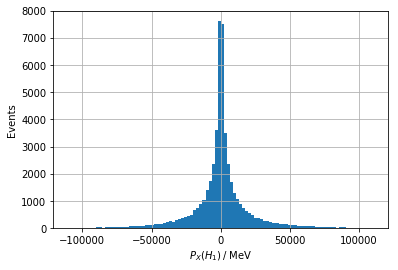
\includegraphics[width=\linewidth]{plots/sim_px_kaon1.png}
    \label{fig:px}
  \endminipage\hfill
  \minipage[c]{0.32\textwidth}
    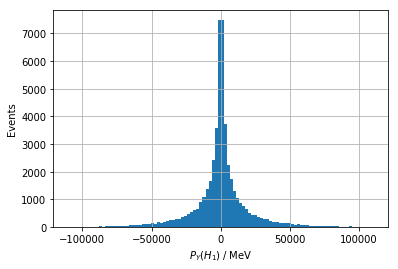
\includegraphics[width=\linewidth]{plots/sim_py_kaon1.png}
    \label{fig:py}
  \endminipage\hfill
  \minipage[c]{0.32\textwidth}
    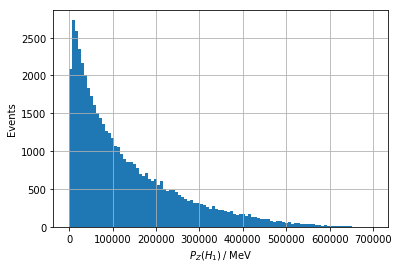
\includegraphics[width=\linewidth]{plots/sim_pz_kaon1.png}
    \label{fig:pz}
  \endminipage
  \caption{Die Impulse in x, y und z Richtung von Kaon1.}
  \label{fig:momenta}
\end{figure}

Es ist in Abbildung \ref{fig:momenta} zu erkennen, dass die Teilchen stark in z-Richtung geboostet sind, was auch zu erwarten ist bei B-Mesonen.

Um die invariante Masse zu berechnen, wird zun\"achst die Energie der B-Mesonen bestimmt.
\begin{equation}
  \symup{E}(B^{\pm}) =
  \sqrt{\left(\sum_{i = 1}^{3} \vec{\symup{p}}_i\right)^2 + \left(\sum_{i = 1}^{3} \symup{m}_i\right)^2}
\end{equation}

F\"ur die Massen wird die Massenhypothese der Kaonen eingesetzt, da dies der interessante Endzustand ist.

Mit der berechneten Energie kann durch umstellen von Gleichung \eqref{eqn:relativityEQ} auf den Impuls und damit auch auf das Betragsquadrat der B-Mesonen geschlossen werden.

In Abbildung \ref{fig:invMassB} liegt der Massenpeak bei etwa $\SI{5279.2}{\mega\electronvolt}$, was sehr eng an dem Wert des PDG liegt.
%Hier müssen wir noch eine Quelle zur PDG Masse einfügen
Dieser Peak ist so scharf, da es sich hier im simulierte Daten handelt. In Wirklichkeit sollte der Peak breiter gefächert sein.

\begin{figure}[!htb]
  \centering
  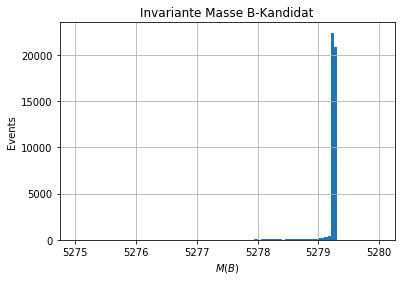
\includegraphics[width=0.8\textwidth]{plots/sim_inv_masse_B.png}
  \caption{Invariante B Masse in den simulierten Daten.}
  \label{fig:invMassB}
\end{figure}

\subsection{invariante Masse der B-Mesonen in echten Daten}
Als n\"achstes wird die invariante Masse der echten B-Mesonen rekonstruiert.
Hierzu wird zun\"achst eine Vorselektion durchgef\"uhrt um den oben genannten Endzustand zu verwenden.
Dazu verwenden die folgenden Schnitte.
\begin{enumerate}
  \item \texttt{H1\_isMuon} == False
  \item \texttt{H1\_ProbPi} < 0.5
  \item \texttt{H1\_ProbK} > 0.5
\end{enumerate}

Diese Schnitte werden analog auch f\"ur Tochterteilchen 2 und 3 angewandt.
Die Verteilungen der Wahrscheinlichkeiten ob ein Endzustandsteilchen ein Kaon oder Pion ist werden geplottet um die Schnitte auf \texttt{H1\_ProbK} und \texttt{H1\_ProbPi} sch\"arfer zu machen falls nötig.
Dies hat zur Folge, dass sehr viel Statistik Im Signal verloren geht und noch ziemlich viel Hintergrund vorhanden ist. Deswegen werden die Schnitte wie oben belassen.

Anschlie\ss end wird, wie schon bei den simulierten Daten, die invariante Masse der B-Mesonen berechnet. Diese ist in Abbildung \ref{fig:realBMass} dargestellt. Um den Massenplot f\"ur die $B^{-}$ von den $B^{+}$-Mesonen zu separieren werden die Ladung der Tochterteilchen multipliziert. Ist das Produkt $+1$,wird das Ereignis zu den $B^{-}$ gez\"ahlt, andernfalls zu den $B^{+}$.

\begin{figure}[!htb]
  \centering
  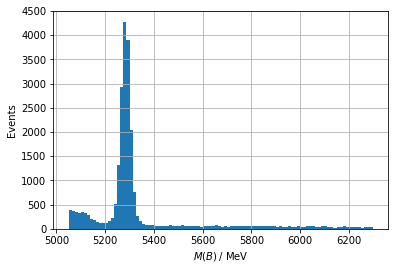
\includegraphics[width=0.8\textwidth]{plots/real_data_inv_masse_B.png}
  \caption{Invariante B Masse in den echten Daten.}
  \label{fig:realBMass}
\end{figure}
